\section{Diskussion}
\label{sec:Diskussion}

Zusammenfassen kann man sagen, dass die Ergebnisse stark von den Erwartungen abweichen.
\newline
Für die Schallgeschwindigkeit in Acryl wurde ein Wert von $\SI{1378}{\meter\per\second}$ ermittelt. Dieser weicht um 98,1\% vom Literaturwert von
$\SI{2730}{\meter\per\second}$ ab. Eine solche Abweichung ist nur durch einen systematischen Fehler in der Bestimmung zu erklären.
\newline
Ansonsten ist zu Bemerken, dass die bestimmten Positionen und Größen der Störstellen für die Großen einen kleineren Fehler aufweisen, als für die Kleinen.
\newline
Bei der Untersuchung des Brustmodels konnte auch nach mehreren Versuchen keine Aufnahme erstellt werden, von der abzusehen war, um welche Art von Tumor es
sich handelt. Obwohl ein gewisser Größenunterschied der Tumore zu spüren war, gelang es nicht, diesen auch durch einen Scan sichtbar zu machen.

\printbibliography{}

\section*{Anhang}
\label{Anhang}

\begin{figure}[H]
    \centering
    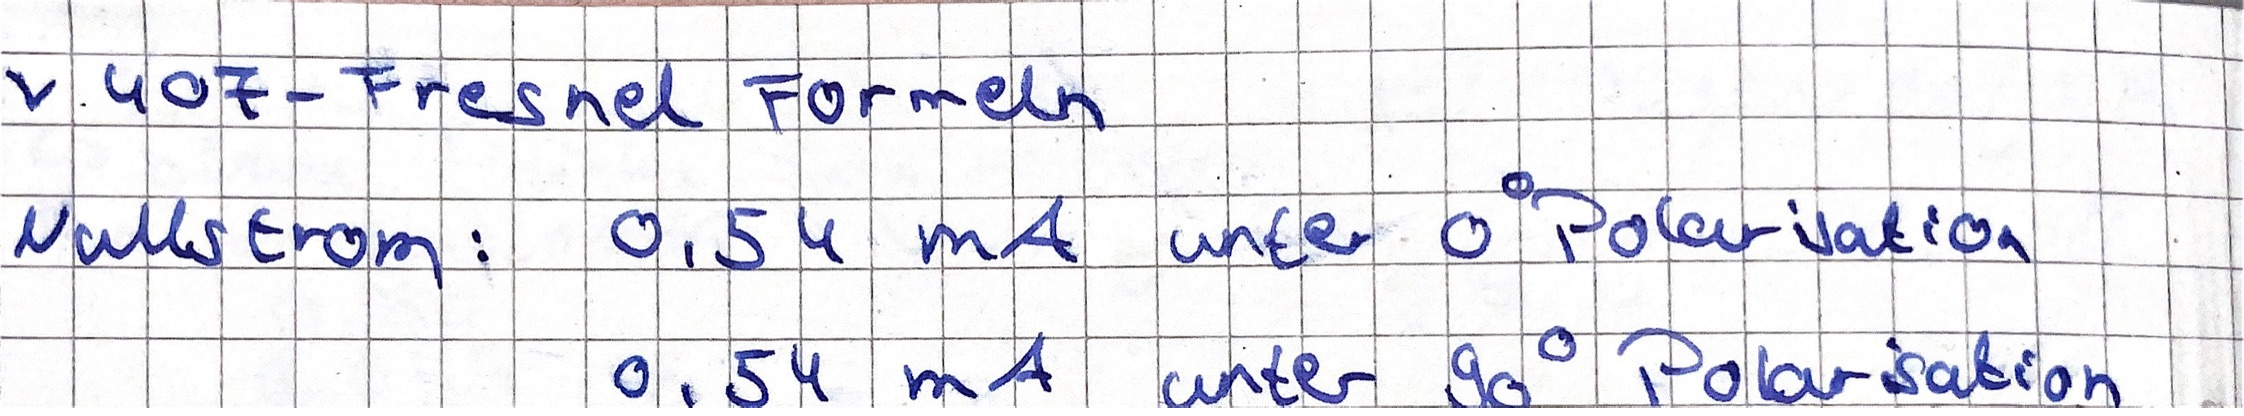
\includegraphics[width=0.5\textwidth]{data/origDaten1.png}
    \caption{Orgininale Messdaten.}
    \label{fig:origDaten1}
\end{figure}

\begin{figure}[H]
    \centering
    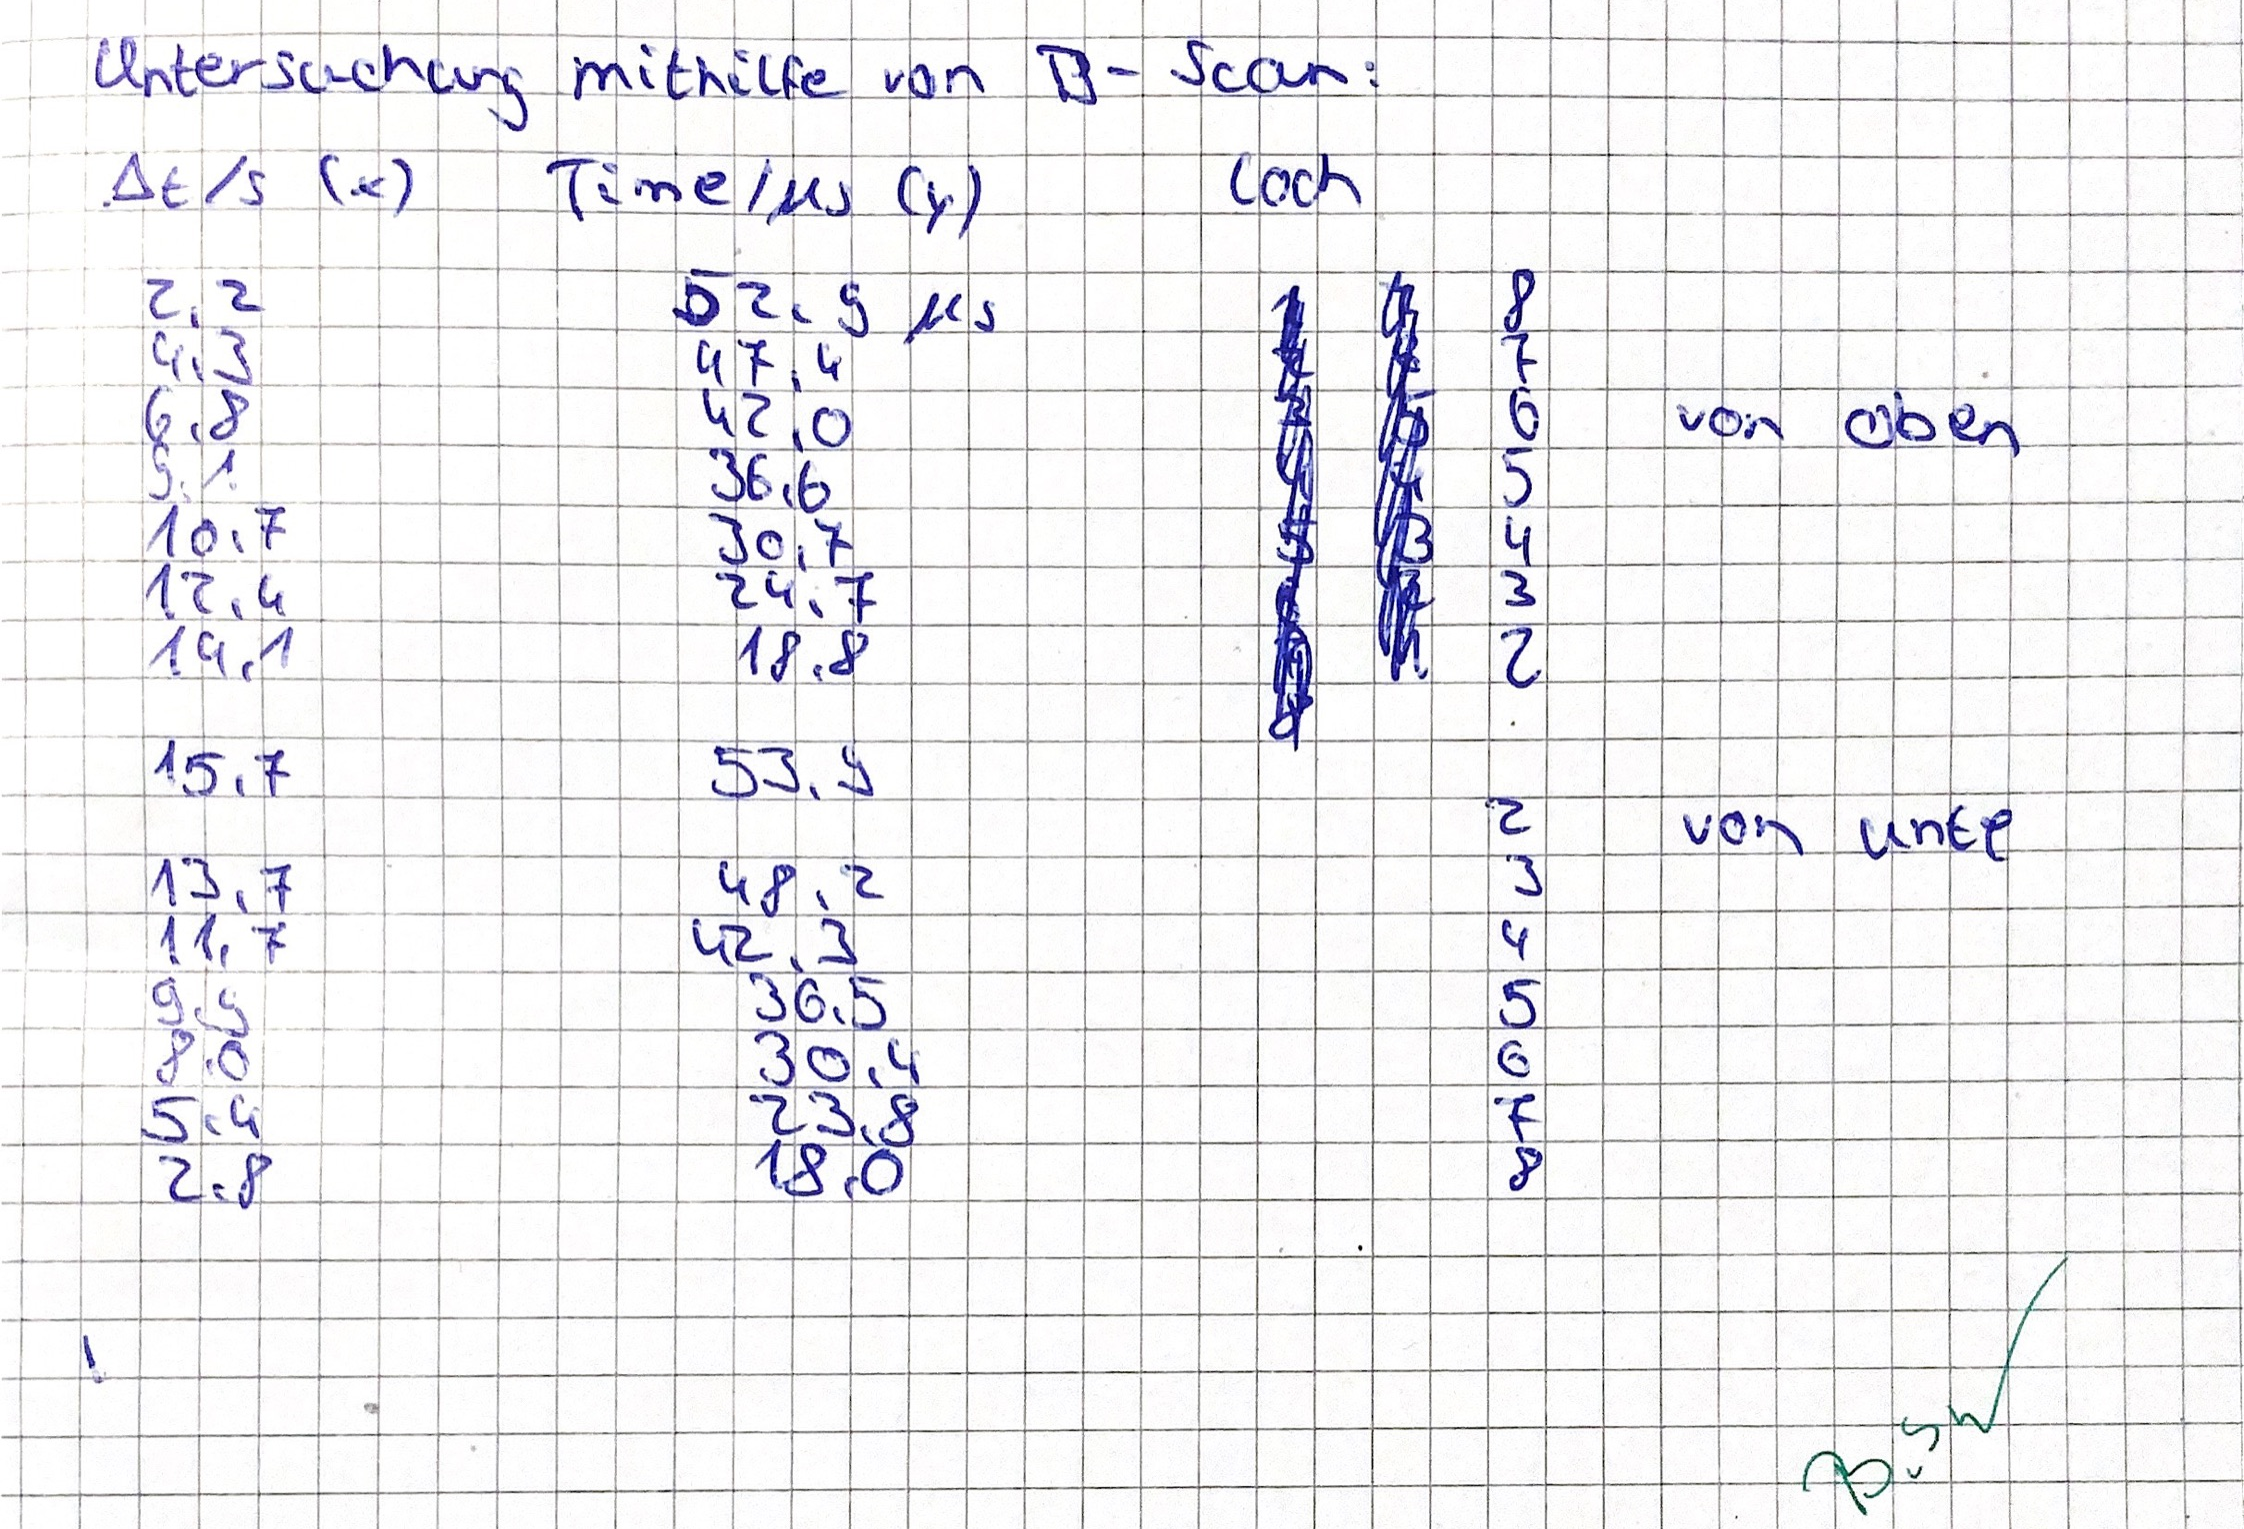
\includegraphics[width=0.5\textwidth]{data/origDaten2.png}
    \caption{Orgininale Messdaten.}
    \label{fig:origDaten2}
\end{figure}